\subsection{Diagrammi delle classi}
\subsubsection{View}
\begin{figure}[hb]
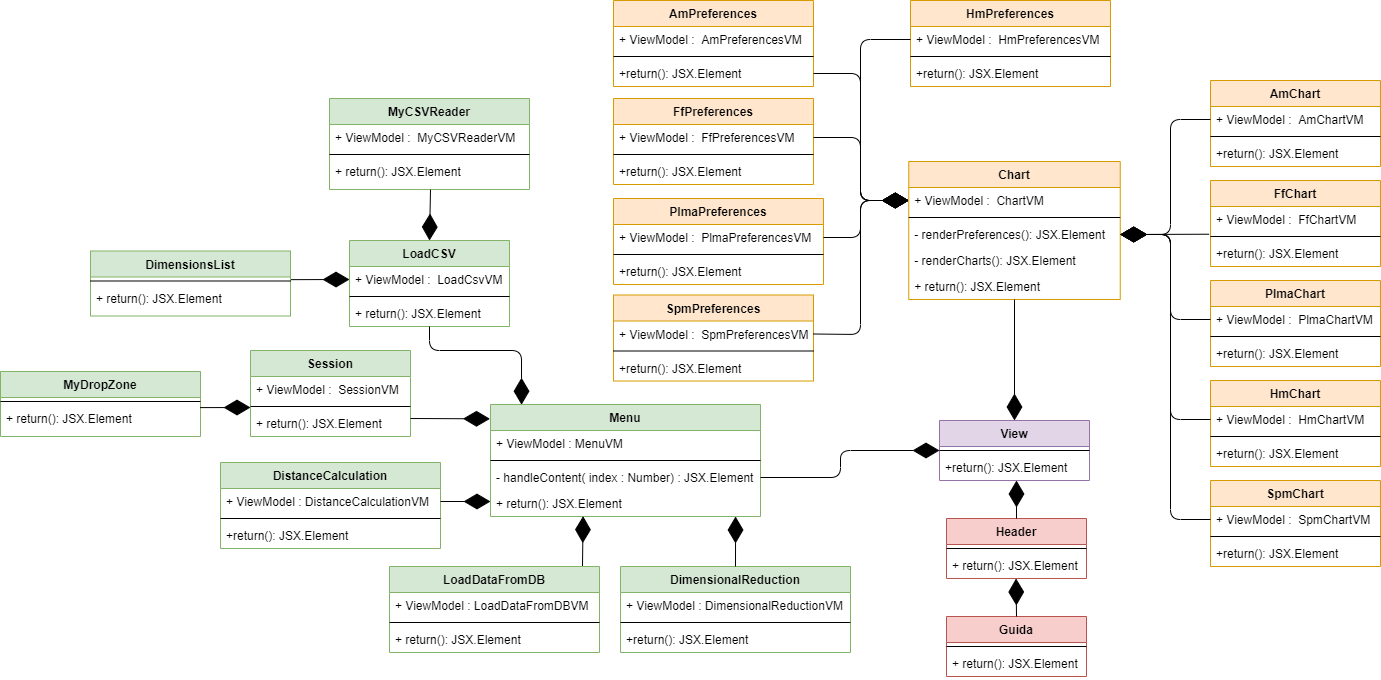
\includegraphics[width=\linewidth]{Images/Allegato Tecnico-Class View}
\centering
\caption{Diagramma delle classi della vista}
\end{figure}
Il diagramma delle classi della vista è costituito da tutti i componenti React che compongono l'interfaccia utente di \NomeProgetto{}.
Visitando dall'alto la gerarchia di componenti, il padre è \textbf{View}, il quale crea l'\textbf{Header} e i più importanti \textbf{Menu} e \textbf{Chart}. Riguardo a quest'ultimi due componenti:
\begin{itemize}
	\item Menu rappresenta per l'utente il punto d'accesso a tutte le funzionalità fornite dall'applicazione. Da qui sono infatti accessibili le finestre per il caricamento dei dati da file CSV (\textbf{LoadCSV}) e dal database (\textbf{LoadDataFromDB}), per il calcolo della distanza (\textbf{DistanceCalculation}), per la riduzione dimensionale (\textbf{DimensionalReduction}) e per il caricamento di una precedente sessione o il salvataggio di quella attuale (\textbf{Session});
	\item Chart è il componente che crea i grafici (\textbf{\textit{NomeVisualizzazione}Chart}) e le relative form per settarne le preferenze (\textbf{\textit{NomeVisualizzazione}Preferences}). La scelta del grafico da visualizzare avviene dal Menu e comprende Scatterplot Matrix, Adjacency Matrix, Force Field, Heatmap e PLMA.  
\end{itemize}
La maggior parte dei componenti hanno un attributo ViewModel: questo indica che hanno una dipendenza verso di esso, usata per ottenere le informazioni di cui hanno bisogno contenute negli store (per esempio i dati o le dimensioni), oppure solo come contenitore della propria \textit{presentation logic}. \\
In questo modo la vista risulta essere completamente separata dalla \textit{business logic} e si occupa solo di ritornare i vari elementi HTML che la costituiscono. 

\newpage
\subsubsection{Model}
\begin{figure}[hb]
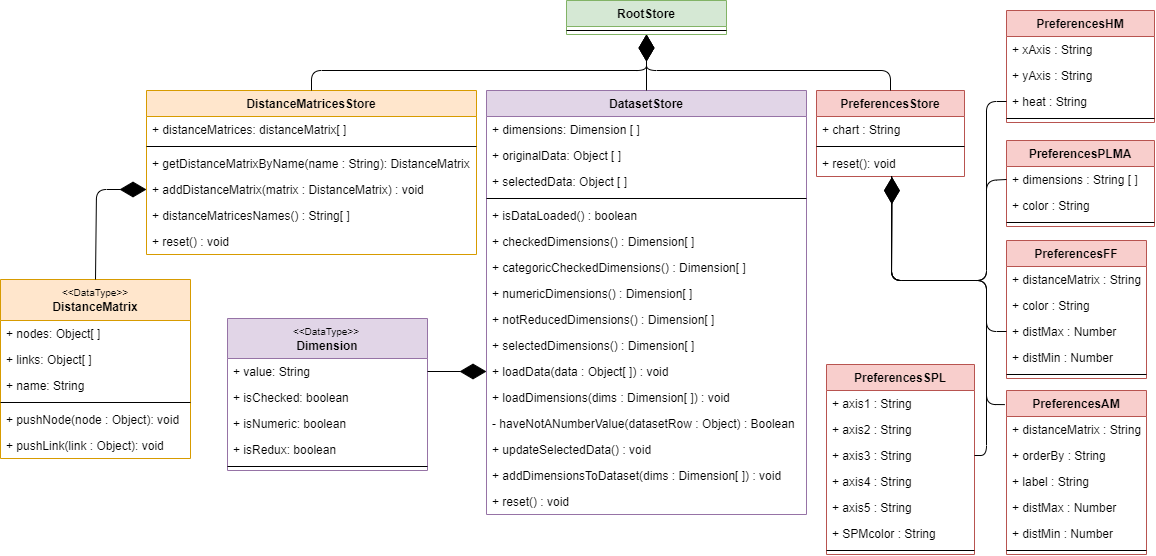
\includegraphics[width=\linewidth]{Images/Allegato Tecnico-Store}
\centering
\caption{Diagramma delle classi del modello}
\end{figure}
Il diagramma delle classi del modello è costituito da un \textbf{RootStore}, il quale istanzia i tre store utilizzati in \NomeProgetto{}:
\begin{itemize}
	\item \textbf{DatasetStore} che contiene i dati caricati e le dimensioni da visualizzare, fornendo i metodi per recuperarli e aggiornarli;
	\item \textbf{PreferencesStore} che conserva le preferenze di visualizzazione di tutti i grafici utilizzati dall'utente; 
	\item \textbf{DistanceMatricesStore} che contiene le matrici delle distanze.
\end{itemize}
\textbf{Dimension} e \textbf{DistanceMatrix} sono i tipi che definiscono rispettivamente le dimensioni e le matrici delle distanze create dall'utente attraverso le varie funzioni di calcolo della distanza fornite (Euclidea, Chebyshev, Manhattan e Canberra). \\ \mbox{}\\
\textbf{PreferencesSPM}, \textbf{PreferencesFF}, \textbf{PreferencesAM}, \textbf{PreferencesPLMA}, \textbf{PreferencesHM} sono i tipi che definiscono le preferenze dei diversi grafici.
Gli store contengono gli attributi \glo{observable} che, nel momento in cui vengono modificati, grazie all'utilizzo di MobX, causano la rirenderizzazione dei componenti \glo{observer} della vista. 

